\clearpage
\section{Setting up ROS for mapping}

During the initial stages of using ROS we attempted to get the installation up and running on the raspbian operating system for the Raspberry Pi. During the gathering of the different necessary packages needed for ROS, some unforeseen issues were encountered. Specifically the GMapping package caused some issues, since it required Python 2.7.1 and upwards. Even though a python version fitting the requirement was installed by default on the raspbian, the GMapping package would not recognize it. Through troubleshooting it was then discovered that GMapping was looking for Python-2.7.1-ubuntu, instead of the Python-2.7.1-debian that was installed together with the Raspbian operating system.

Instead of continuing to deal with the ROS issues on the raspbian installation, Ubuntu ARM was instead installed on the Raspberry Pi.
The installation process using Ubuntu ARM was much faster and more fluent compared to installing ROS on the raspbian installation. During the installation of ROS on Ubuntu a new package named Hector-slam was discovered. 
%TODO add additional information here
This package allows ROS to generate a map without the use of the GMapping package. Its biggest advantage is that it does not rely on odometry to know whether the reference frame has changed.

\subsection{something}
During our development, we gained a deep understanding of how all the moving parts in ROS work together.


\begin{figure}[H]
	\centering
	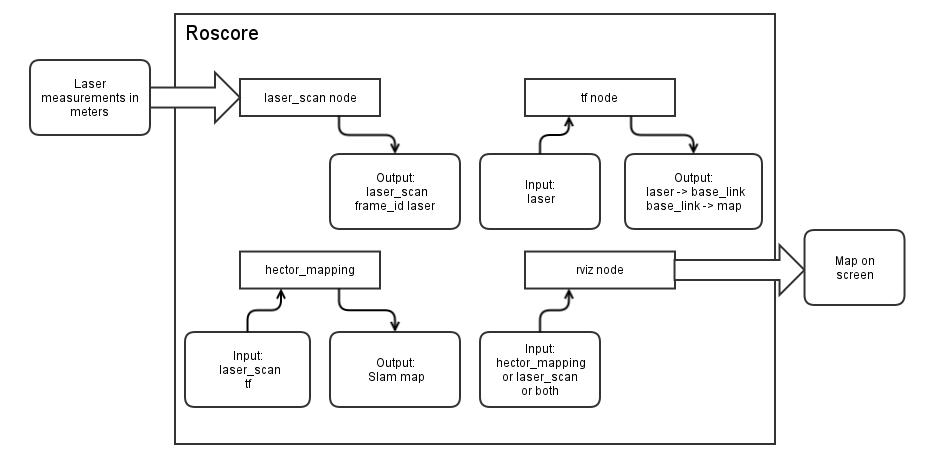
\includegraphics[width=.8\linewidth]{images/ROSflow.png}
	\caption{Ros flow}
\end{figure}

Roscore is the main process behind ROS. It allows for all running nodes to talk to each other. By itself it does nothing.

Nodes are the smalles pieces of ROS that are put together to form a full aplication. They are run as separate applications, all with their own executable files. The only way nodes communicate is through roscore. To make a node, it is necessary to use the ROS library in whatever programming language is chosen.

Roslaunch is the ROS command that allows starting multiple nodes, and also allows giving parameters to nodes. Roslaunch executes nodes that are specified in an XML file you give it, called the launchfile.
%our launchfile here

\subsection{something else}
During this stage of testing, ROS gathers the data and generates the map directly on the Raspberry Pi. The Raspberry Pi is accessed through SSH and the generated map is then broadcast to computer through the SSH connection.

\begin{figure}[H]
	\centering
	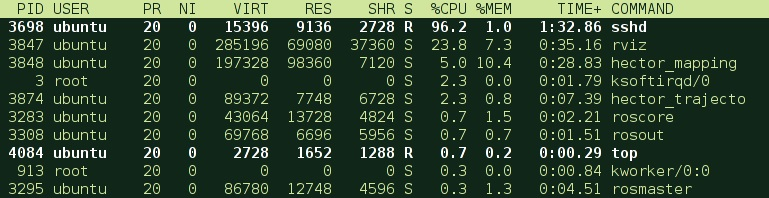
\includegraphics[width=.8\linewidth]{images/rvisScreenshotCropped.jpg}
	\caption{The resource usage}
\end{figure}


After testing the Hector-slam some lag issues were experienced, which seemed to be caused by multiple things: One thing could be that generating the map on the actual Raspberry Pi required too many resources from the CPU, another could be that the transfer of the visualization to the computer screen required more bandwidth than there could be supplied.

%TODO Needs expanding?
To reduce the amount of resources used by the Raspberry Pi, the map needs to be generated and visualized using separate computing unit. ROS is built to have separate nodes with a main computing unit.

